%----------------------------------------------------------------------------------------
%	PACKAGES AND OTHER DOCUMENT CONFIGURATIONS
%----------------------------------------------------------------------------------------

\documentclass[twoside,fontsize=12pt]{article}
%\documentclass[oneside]{article}
\usepackage{lipsum} % Package to generate dummy text throughout this template
\usepackage{graphicx}

%\usepackage[sc]{mathpazo} % Use the Palatino font
\usepackage[T1]{fontenc} % Use 8-bit encoding that has 256 glyphs
\linespread{1.5} % Line spacing - Palatino needs more space between lines
\usepackage{microtype} % Slightly tweak font spacing for aesthetics
\usepackage{listings}
\usepackage[hmarginratio=1:1,top=32mm,columnsep=20pt]{geometry} % Document margins
%\usepackage{multicol} % Used for the two-column layout of the document
\usepackage[hang, small,labelfont=bf,up,textfont=it,up]{caption} % Custom captions under/above floats in tables or figures
\usepackage{booktabs} % Horizontal rules in tables
\usepackage{float} % Required for tables and figures in the multi-column environment - they need to be placed in specific locations with the [H] (e.g. \begin{table}[H])
\usepackage[hidelinks]{hyperref} % For hyperlinks in the PDF

\usepackage{lettrine} % The lettrine is the first enlarged letter at the beginning of the text
\usepackage{paralist} % Used for the compactitem environment which makes bullet points with less space between them
\usepackage{chngcntr}
\counterwithout{figure}{section}
\usepackage{abstract} % Allows abstract customization
\renewcommand{\abstractname}{}    % clear the title
\renewcommand{\absnamepos}{empty}
\renewcommand{\abstractnamefont}{\normalfont\bfseries} % Set the "Abstract" text to bold
\renewcommand{\abstracttextfont}{\normalfont\small\itshape} % Set the abstract itself to small italic text
\usepackage[super, sort&compress]{natbib}
\setlength{\bibsep}{0.0pt}
\bibliographystyle{unsrtnat}
\usepackage{titlesec} % Allows customization of titles
\renewcommand\thesection{\Roman{section}} % Roman numerals for the sections
\renewcommand\thesubsection{\Roman{subsection}} % Roman numerals for subsections
\titleformat*{\section}{\LARGE\scshape\centering}
\renewcommand{\bibsection}{\section*{\refname}}
\titleformat{\section}[block]{\LARGE\scshape\centering}{\thesection}{1em}{} % Change the look of the section titles
\titleformat{\subsection}[block]{\large\bfseries}{\thesubsection}{1em}{} % Change the look of the section titles
\titleformat{\subsubsection}[block]{\bfseries\textit}{\thesubsubsection}{0.1mm}{} % Change the look of the section titles
\usepackage[table,xcdraw]{xcolor}
\usepackage{caption}
\renewcommand{\thefootnote}{\fnsymbol{footnote}}
\usepackage{setspace}
\captionsetup[figure]{font={stretch=1}}
\usepackage{fancyhdr} % Headers and footers
\pagestyle{fancy} % All pages have headers and footers
\fancyhead{} % Blank out the default header
\fancyfoot{} % Blank out the default footer
\fancyhf{}
\renewcommand{\headrulewidth}{0pt}
%\fancyhead[C]{Running title $\bullet$ November 2012 $\bullet$ Vol. XXI, No. 1} % Custom header text
\fancyfoot[RO,LE]{\thepage} % Custom footer text

%----------------------------------------------------------------------------------------
%	TITLE SECTION
%----------------------------------------------------------------------------------------

\title{\vspace{-15mm}\fontsize{18pt}{10pt}\normalfont\textbf{Understanding the functional effects of structural variation in non-coding regions.\\ \vspace{4 mm} {{\footnotesize \textit{Analysing multi-level 'omics using graph-based integration methods.}}}}} % Article title

\author{
\large
\textsc {RHWE (Robin) van der Weide}\thanks{Promotor: Prof. Edwin Cuppen, PhD | Copromotor: Joep de Ligt, PhD}\\[2mm] 
\normalsize  BSc. Biology\\
\normalsize  MSc. Cancer Stem cells \& Developmental biology (honours program)\\
\normalsize  Utrecht Graduate School of Life Sciences \\
%\normalsize \href{mailto:john@smith.com}{john@smith.com} % Your email address
\vspace{-5mm}
}
\date{}

%----------------------------------------------------------------------------------------

\begin{document}

\maketitle % Insert title

\thispagestyle{fancy} % All pages have headers and footers

\newpage
\renewcommand{\abstractname}{\begin{center}
Summary of the research
\end{center}}    % clear the title

\begin{abstract}
\noindent
Effects of structural variation in the non-coding regions of the human genome are rarely studied which is strong contrast to their known role in disease\cite{Weischenfeldt2013}. Systematic approaches for elucidating their functional effects are rarely successful, mainly due to the complexity of non-coding regions (e.g. \textit{cis}- and \textit{trans}-acting elements, co-activation, non-coding RNA interaction). Predictions on functionality are further complicated by the diversity in types and consequences of structural variants. Integration and visualisation of complex, multi-layered datasets are needed to better understand the functional effects of these events\cite{Munoz2011}.
\medskip

\noindent 
Within the realm of systems biology, graph-based approaches are well-known and -used for analysis of interaction-networks. The main benefits of abstracting complex data-sources to graphs are enhanced exploratory analysis via visual analytics and integration of datasets of different levels and dimensions. The ongoing cost reduction of various 'omics-approaches coupled to high throughput research, has led an explosion of available data. However, the complexity of integrating and analysing these large datasets increases with every added 'omics-layer or dimension (e.g. time-series, treatments). 

For larger and more complex datasets like these, the bioinformatics community -following other \textit{big data} sciences- is starting to gravitate towards the Resource Description Framework (RDF). This is a simple and flexible graph-integration approach, which also allows for easy connection to (web-based) public repositories. The formation and testing of hypotheses on these created and/or combined networks is made straightforward by using simple SPARQL-queries and subsequent visual analytics-methodologies.
\medskip

\noindent Here, we propose the use of graph-based methods to decrease the complexity of integrating and visualizing multi-level and -dimensional biological data. By integrating patient-derived data of the UMC Utrecht, we are in the premier position to uncover new biological insights into the complex biology of non-coding structural variants. Our resulting methodologies and discoveries could aid a large community of both scientists and patients, by enabling further elucidation in congenital disease and cancer. 
\end{abstract}
\medskip

\noindent \textbf{Keywords:} graph-based methodology, structural variation, multi-level data integration, non-coding genomics

%----------------------------------------------------------------------------------------
%	ARTICLE CONTENTS
%----------------------------------------------------------------------------------------
\newpage

\section*{Background}
%\subsection*{	big data: weinig systematisch over NC,laat staan sv}
%Er is veel data om te gebuiken! Maar het is wel erg veel... en heterogeen
The amount of (public) biological data has exploded in the last years (even outpacing Moore's law\footnote{A two-fold in- or decrease of a variable (here: dollar/nt) per two years.}). This is the result of the advances in omics-technologies like Next-Generation Sequencing (NGS) and Mass-Spectrometry (MS), in both performance and costs. The addition of other dimensions, like time-series or treatments, is a second factor for the highly complex nature of current biomedical research. While there are plenty of studies on single-level data analysis, both academia and industry agree that data-integration is essential to understanding the complex nature of biology more thoroughly \citep{Gomez-Cabrero2014, Huttenhower2010, Searls2005, Hamid2009}. 

The vast majority of large-scale integrative studies have been conducted on the coding-regions of the genome\cite{ENCODE}. Although finding functional genetic variation in the protein-coding regions of the genome has thus been the focus, these regions amount only to approximately two percent of the genome\cite{Lander2001}. Of the remaining 98\%, approximately 6.2\% is theorized to be biologically functional (i.e. is under negative evolutionary pressure)\cite{Rands2014}. One of the primary reasons behind this focus is the relative uncomplicated nature of studying coding regions, as consequences on lower levels (e.g. transcription, proteins) are linearly traceable\cite{McLaren2010}. 

This is in contrast to the non-coding regions, which often do not show a linear effect on other levels\cite{Bird2006}. A good illustration of the complexity of the non-coding regions is the ENCyclopedia Of DNA Elements (ENCODE)-project\cite{ENCODE}, which contains over fifty different signals (e.g. histone methylation, DNase1 hypersensitivity). The fact that non-coding regions have roles in the regulation of both close and distant genes (i.e. \textit{cis-} and \textit{trans-}acting) provides even more complexity to the analysis of structural variants (SVs) in these regions. For example, the Pierre Robin Syndrome (PRS): SVs (deletions or duplications) in the 3Mb surrounding the SOX9-gene in particular tissues are causative of the striking phenotype of undeveloped mandibles and tongue in children\cite{Benko2009,Kurth2009}. 
\medskip

\noindent
%\subsection*{	wat valt er te halen? uitleg NC}
%Non-coding: lastig en weinig onderzocht
% Grootste winst is te halen in het combineren van lagen (distant relationships)
Genome-Wide Association Studies (GWASs) on a broad range of congenital and acquired diseases (e.g. cancer) have shown that non-coding locations are associated with these diseases. This -of course- to be expected, with the discoveries of various functions of the non-coding regions: from (in)directly regulating the transcription-machinery, to playing mayor roles in mRNA-degradation and from post-transcriptional modifications, to directly affecting the localisation of the transcript\cite{Pichon2012,Barrett2012}. Pseudogenes are also categorised as non-coding, but can be resurrected by gene conversion due to structural variants\cite{Kidd2010}. Pseudogenes can perform as decoy for their coding homologs\cite{Poliseno2010} (as was found to be the case in both oncogenes and tumour suppressors) and lead to RNA-interference by pseudogene-transcribed endo-siRNAs\cite{Tam2008}.

Until 2013, however, tools and sources to systemically explore and analyse the functional consequences of variations in non-coding genomic regions were limited. In the last two years, several advances have made it possible to assess the consequences of individual variations in non-coding regions\cite{Ongen2014,Khurana2013}. Studies on cancer-specific causative non-coding variation are beginning to emerge in the last two years, including colorectal- and skin-cancer\cite{Ongen2014,Huang2013}, and computational methods for non-coding regions are just starting to come up in the literature of 2014\cite{Khurana2013,Kircher2014}. %However, no large-scale integrative studies have been performed, which is partly due to the current state of integrative methods. 
\medskip

\noindent
%\subsection*{hoe valt dit te halen? (graphs: integratie en visualisatie)}
%Distant relationships vindt je het makkelijkst met een graph
However, only a few layers and dimensions have been integrated per study and results are -for the most part- cherry picked, instead of systematic. This is mainly due to the methods used in integration-studies: most of them are set up in the same manner as individual-level experiments, whereafter they are combined. These methods are limited due to the large amounts of parsing-time (i.e. the time to convert various file/region-formats). An example of the large amount of analytical time needed, when using these methods is the study of \citet{Munoz2011}: every two months of data-accumulation costed two years of analysis.

The limited number of truly integrative studies use computational approaches to reconstruct biological networks. While a valid strategy, scaling the analysis from the bacteria used by \citet{Karr2012} and \citet{Lerman2012} to multi-cellular organisms proves to be difficult. The most obvious reasons for this are the complexity of the used mathematical methods, the integration of multiple data-sources (with varying file-formats) and the use of an inflexible database-structure.
%\subsection*{	big data graph-methods}
%wat is er hier al gedaan en wat nog niet?
%Waar stond RDF vijf jaar geleden? En waar staat RDF nu?
%VA is nodig en heul handig, ook voor leken
\medskip

\noindent
To overcome these (scaling) issues, we propose the use of graph-based integration methods. The most apparent method for this is from the semantic Web: the \textit{Resource Description Framework} (RDF) and its query-language \textit{Sparql Protocol and RDF Query Language} (SPARQL). RDF is a general and simple framework for making statements about subjects, already heavily used in big data science, enabling users to integrate and search data based on semantics. Every RDF-statement (i.e. a triple) has three parts: a subject, a predicate and an object (e.g. \lstinline|BRAF1 :: molecular function :: calcium ion binding|). This makes it possible to abstract and link every object to another and denote the relationship between them: there is no need for additional (file)formats. By linking triples to each other by either a common object or subject (essentially constructing a graph-based network), new relationships can be inferred (fig.\ref{fig:rdf}). Aside from the non-complex, flexible and self-describing nature of the RDF-data, triples can be seen as a modular directed graph: users can connect multiple (remote) relevant RDF-sources (e.g. UniProt and Proteomics-data). Every additional RDF-source results in a more relevant and heterogeneous population of triples, making the network more complex and informative. 


\newpage
There have been various studies on the integration of biological signals with the aid of semantic web technologies: the power of ontology-based entailment\footnote{The logical consequence of having two linked ontologies, thereby inferring an additional, encompassing relationship on the shared object/subject} reasoning is widely acknowledged\cite{Sahoo2008}. However, the momentum was lacking: until 2014, big databases were not available in RDF-format. This meant that bioinformatical research, using graph-based methodology through RDF, had little to no outside support, as they could only integrate proprietary data. An example of this are the methods used in microarray analyses by \citet{Szpakowski2009} in 2009. Recently, EMBL-EBI has opened their RDF-platform, boasting six big data-sources (Gene Expression Atlas, ChEMBL, BioModels, Reactome, BioSamples and UniProt)\cite{Jupp2014}. This was the boost needed to further incorporate graph-based integration via RDF in biological analyses.
\medskip

\begin{figure}[H]
    \centering
    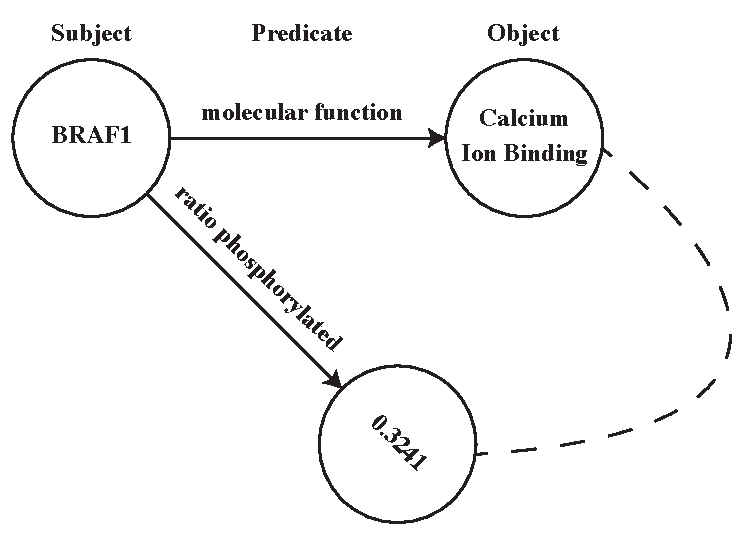
\includegraphics[width=0.8\textwidth]{rdf.pdf}
    \caption{\textbf{General outline of RDF.} \textbf{A}) By linking two triples by their common subjects, \textbf{B}) one can infer the relationship between the two objects via the predicates and find patterns%: a gene, responsible for calcium ion binding, has a low phosphorylation level in the investigated sample
    .}
    \label{fig:rdf}
\end{figure}
\noindent
Extracting relevant information from this "hairball" of linked objects and subjects has been an important issue and challenge since the beginning of big data, as \citet{Pavlopoulos2008} stated in 2008. SPARQL provides the ability to filter on an arbitrary number of (human-readable) expressions and can combine multiple databases to query, like the RDF-databases of EMBL-EBI \citep{Jupp2014}. Another advantage of using SPARQL is the increase in scalability by including multiple triplestores in the same query. By enabling the use of small and specific triplestores, such a federated query results in faster retrieval of the data.

Combining these improvements in searching and linking networks with web-based visual analytics will create a paradigm shift in the way integrative analysis of (biological) data is done. Visual analytics has been shown to result in the most optimal analysis-effectivity as it allows the user to combine the data with their own background and intuition %(fig. \ref{fig:ae})
. Not only can data be more effectively analysed, but it can also be better understood and presented, due to the ability to provide an overview of the complete dataset\cite{Thomas2005, Keim}. 
%\begin{figure}[h!]
%    \centering
%    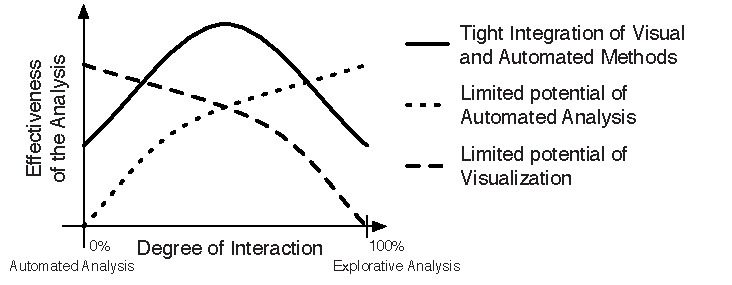
\includegraphics[width=0.5\textwidth]{autoVSexplo.pdf}
%    \caption{\textbf{Trade-offs between automated and explorative analysis.} By combining automated analyses with the background and intuition of the user, an optimal amount of effectivity can be attained. Picture taken from \citet{Keim}.}
%    \label{fig:ae}
%\end{figure}
\newpage
\section*{Preliminary studies}
During my Masters studies, I have already implemented graph-based methods for different purposes. As an illustration of the strengths of multilayer network-analysis, I describe a small example from the work I have done as an intern an the Sanger Institute\footnote{Unpublished data, discretion appreciated.}. Furthermore, we show trough a pilot-study the added efficiency of our proposed methods.
\subsection*{Cis-regulatory regions: potential}
When analysing predicted altered and/or de novo transcription factor binding sites (TFBS) by single-nucleotide polymorphisms (SNPs) in non-coding regions of over 1300 melanoma-patients, no overrepresented TFBS were found. We then discided to use graph-based data integration methods by linking the SNPs to regions in the TF-ChIP data of ENCODE\cite{ENCODE}. Furthermore, two triple stores were added: TcoF -containing TF-interacting proteins and co-factors- and gene ontology terms form the GO consortium. We found that there was a clear overrepresentation of TFs binding to transcription co-activators, like NCOA6, which have a functional role in \emph{\lstinline|vitamin D receptor binding|}. Further analyses showed more evidence of the importance of these findings in familial melanoma (e.g. co-segregation in melanoma-prone families). Without the multilayer network-analysis, in this case of genomics and epigenomics data, such new testable hypotheses are often not found. And without RDF, different databases and -sources would be much harder to integrate for (exploratory) analyses. 
\begin{figure}[H]
    \centering
    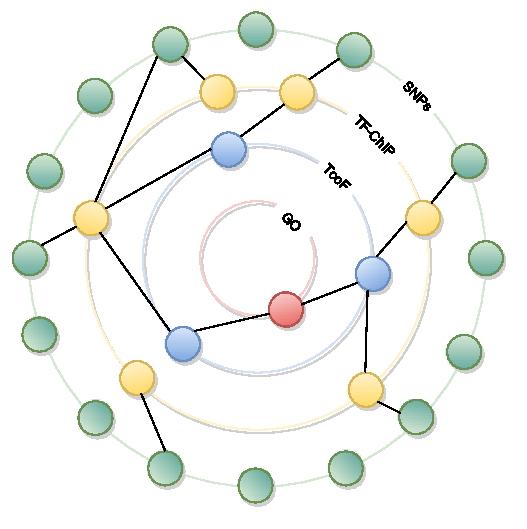
\includegraphics[width=0.425\textwidth]{rondjeGraphs.pdf}
    \caption{\textbf{Graph of GO:0042809.} From a large dataset of mutations in melanoma-patients (outside ring) to a new -testable- hypothesis, alteration in vitamin D receptor binding (inside ring), via a TFBS-regions and a TF-protein interaction database.}
    \label{fig:mela}
\end{figure}
\subsection*{Ribosomal profiling and gene ontology: logistic efficiency}
A small-scale pilot-study was performed on the data of \citet{VanHeesch2014}. This dataset includes transcriptome data of mRNA's, bound to a number of ribosomal units (1 to 7+) and matching exome-data. If one would be interested in the molecular functions of a gene with an allelic bias, a disproportional amount of time is lost on parsing, intersecting and downloading various types of data (fig. \ref{fig:awesome_image}). With the conventional methods, twelve set-operations (e.g. intersections, unions) have to be performed on $\pm$5gb of data. Furthermore, three datasets ($\pm$15gb) have to be completely downloaded once -until a new version is launched- before a simple exploratory question can be answered. Approximately three and a half hours was needed to perform this, in contrast to one hour with the proposed methods. Of this hour, more than fifty minutes were used to convert data to a triple-store: every query hereafter takes up approximately 10 minutes. First and foremost, this pilot illustrates the low-complex nature of the proposed methods. Secondly, it shows the valuable property of having a separate query-stage, which results in being able to make more than ($\frac{(8*60)-50}{10}= $) forty queries in eight hours, instead of approximately ($\frac{8-3,5}{3,5}= $) two queries with the currently used methods.
\begin{figure}[h!]
    \centering
    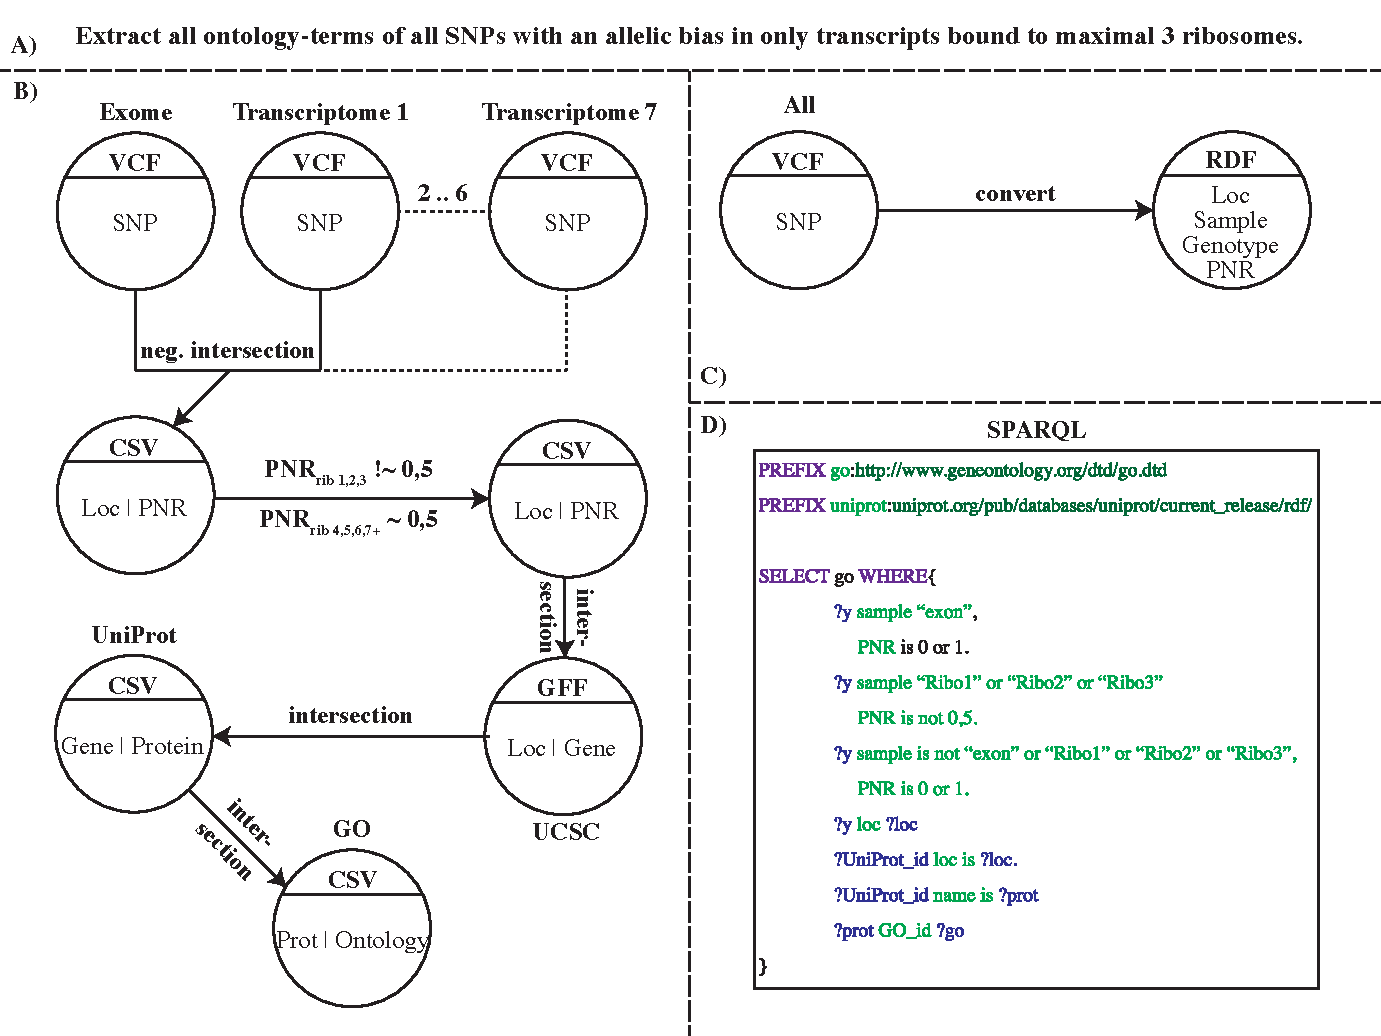
\includegraphics[width=0.85\textwidth]{DifferencesInDoingThings}
    \caption{\textbf{Differences between current integration techniques and RDF.} For a question like \textbf{A}, series of parsing and interception steps are needed ( \textbf{B}). External sources have to be fully downloaded and converted. When using RDF, all data is converted into triples once (\textbf{C}) and subsequent queries can be made in SPARQL (\textbf{D})%, incorporating relevant outside sources, which can be easily changed without having to juggle/download the data again
    .}
    \label{fig:awesome_image}
\end{figure}

\section*{Scope \& aims}
The aim of this project is to create new biological insights in effects of structural variations in the non-coding regions of the genome. For this, a large number of datasets and -sources have to be integrated and analysed. Big data graph-based methods, like RDF,  allow us to do this.
Thus, this proposal has two sub-projects, which rely heavily on each other:

\begin{enumerate}
\item \textbf{Graph-based data integration \& visualisation} 
Generation and adaptation of novel methodologies for integration and analysis of large scale, multi-dimensional biological data. And, more specifically, for structural variants in non-coding regions.
\item \textbf{Multi-level analysis} 
Multi-level and -dimensional integrative analysis to elucidate the consequences of genomic structural variations in non-coding regions, which are found in patients with congenital disease and cancer. 
\end{enumerate}
\section*{Relevance}
The 2014 survey of \citet{Gomez-Cabrero2014} showed that biomedical academics had the highest interest (78.2 percent) in the integration of multiple omics-datasets and that there was a high need for standardized tools and data-types. Data-storage, -exploration and -exploitation were found the be key. Their conclusions were best summarized by \textit{the need for having exploration tools, which combine summary statistics and interactive visualisations, to analyse heterogeneous data-sets}.
\medskip

\noindent
\emph{ \color{red}HIER NOG IETS OVER NON\_CODING\_NC }
\medskip

\noindent
The implementation of our proposed graph-based methods will be swift since RDF already is a web-standard and a significant number of public biology-related sources are already in RDF-format. This will enable users of our methodologies to efficiently connect and integrate their data with public resources. Current statistical software, like the R environment, have packages to extract and further analyse SPARQL-output. This means that users only have to learn SPARQL-queries, in order to use the proposed methods.

By enabling more users to use methods and sources of our approaches, this research will, in a broader perspective, have a direct effect on the semantic web and biological databases. By lowering the (bioinformatical) threshold for analysis, more data can be faster analysed by more people, further accelerating research. Users will also be able to tell their story (i.e. results) better. Psychologist will, for example, be able to get a better visualisation and thus understanding of a neuroscientist's work. Big pharmaceutical companies will be able to further include and analyse data of basic science, clinical trails and business-statistics with more efficiency. Moreover, the research-community will be one significant step further in dissecting the complex biology of (structural variation in) non-coding regions of the genome.

\section*{Experimental strategy}
\subsection*{Placement and institute}
Due to the affiliation with the University Medical Center Utrecht (UMCU), we are in a unique position to test our hypotheses and methods in both research and clinical settings. Furthermore, the HUB-biobank \url{http://hub4organoids.eu/} in the Hubrecht Institute  enables us to perform analyses on organoids, providing us a stable and homogeneous \textit{in vitro} platform for validations in (non)cancer-samples. With the proposed methods, we will be in a position to perform integrative studies with appropriate biological validation on the mechanisms and consequences of (structural) variation. 

Groups in the Hubrecht are heavily involved in (inter)national consortia, like the \textit{Cancer Genomics Centre}. This national consortium of research-groups, predominantly of the Hubrecht Institute and the Netherlands Cancer Institute (NKI), focusses on cancer's (epi)genetic alterations and responses to drugs. Data from this project will include various levels (e.g. (epi)genomics, phospho-proteomics) and dimensions (e.g. drug-responses, time-series). For the cancer sub-population study, a collaboration between the \textit{van Oudenaarden}-group (lineage-tracing and CELL-seq) and the \textit{Clevers}-group (cancer-biobank) will be formed.

A considerable amount of Dutch research groups make use of the Utrecht DNA-sequencing Facility(UDsF) and the Netherlands Proteomics Centre, which ensures adequate opportunities for collaborations and data-integration-based research questions. Furthermore, the newest generation of DNA-sequencing methods from Oxford NanoPore and Pacific Biosciences are being deployed in the UDsF. These technologies result in larger sequenced stretches of DNA, which will make a considerable impact in the identification and analysis of larger structural variants.

Ties with international leaders in biology-related semantic web and visualisation technologies have been made and will continue to be expanded. Joachim Baran and Pjotr Prins have been heavily involved in the planning stages, being key players in handling various data-formats (into RDF) with \textit{BIO-Ruby}. Communications with Artem Tarasov of \textit{Sambamba} and Jerven Bolleman -key engineer of the \textit{UniProt-RDF} project- have also been established.
%!!WGS!!
%Data extraction:
%	BAM ?
%	VCF ?
%Welke sources precies (we moeten keuzes maken, max 3 zou ik zo zeggen)
%	
%!!NanoPore!!
%
%Data integration:
%	Public / Private
%	Epi / HiC / ...   (ook hier specificeren waar we meest verwachten / op focussen / waar 	    het vandaan komt
%
%Organoids
%
%CRISPR / CAS9



\subsection*{Technical themes}
%		RDF: gebruiken wat er is en waar nodig creeren (basis ligt er al, uitbreiden)
%		Visual analytics voor de graphs
Before any analysis on the effects of non-coding structural variants can occur, we firstly lay a strong technical foundation. Not only do we have to develop/adopt bioinformatical approaches, but we have to take into account the need for validation.

The application of graph-based methods will be largely based on the RDF-platform. While biology-related triplestores (RDF-databases), conversion-tools and basic ontologies are already made, we only have to focus on the specific missing elements.
\medskip

\noindent
\textbf{Data usage} \\

\emph{ \color{red}vcf als start (miss fine-mapping van bams).. dus werken post-calling/filtering
databases: encode als leidraad + rdf-dbs}\\

The Cancer Genome Atlas (TCGA) has been translated into a RDF-resource in 2014\cite{Saleem2014}. The atlas includes whole-genome (\emph{Affy SNP 6.0-}) copy-number variation data. The fact that this resource also includes clinical, transcriptomic, epigenomic and proteomic data, makes it a very valuable resource for our experiments.

\emph{ \color{red}stukje over andere databases: EBI, GO, KEGG}



\medskip

\noindent
\textbf{Integration and visualisation} \\
\emph{ \color{red}iets over wat we gaan doen voor visual analytics van de graphs en de mgelijkheid om een centraal -uitbreidbaar-platform te maken voor sparql-queries icm VA. (voortborduren op dingen als Epiviz en rdf:SynopsViz.  http://swui.semanticweb.org/swui06/papers/Karger/Pathetic\_Fallacy.html laat mooi een groot probleem zien: een rdf-hairball zit niemand op te wachten (i.e. de echte graph is dus niet goed voor analyse: VA is nodig: VA is het beste als een browser waarin je lekker op los kan klikken.)}



\medskip

\noindent
\textbf{\textit{In vitro} validation} \\

\medskip

\noindent
\textbf{Validation strategy} \\
\emph{ \color{red}crispr/cas9: mogelijkheid om een select aantal candidates in deatil uit te werken}


\subsection*{Biological themes}
%		Characterisation of the effects of SVs in cis- and trans-regulatory regions in disease. (TFBS, ncRNA, epistasis?)
%		Non-coding structural factors of drug-resistance
%		Single-cell analysis of SVs in cancer sub-populations
This set of questions (ordered descending on $\frac{Pay}{Risc}$) shows the main innovative point of our proposed methods: they enable us to analyse and integrate several 'omics-levels and multiple dimensions (e.g. drug-resistance, cancer types), while allowing easy connection to public data. 
\medskip

\noindent
\textbf{Study recurrent non-coding SVs in public databases} \\
adaasafssf
\medskip

\noindent
\textbf{Identify effects of Chromotripsis induced SVs ??} \\
Wigard heeft data van chromotripsis data patienten die volgens mij deels publiek is.
[ref: Deciphering the pathogenic consequences of chromosomal aberrations in human genetic disease.]
Wij willen dit natuurlijk verder trekken maar is een waardevolle dataset.
\medskip

\noindent
\textbf{Study non-coding SVs in healthy Adult Stemcells} \\
Volgens mij zou Ruben dat helemaal cool vinden ......
\medskip

\noindent
\textbf{Single-cell analysis of SVs in cancer sub-populations} \\
Due to the advances in single-cell sequencing (CELL-seq) of both DNA and RNA, we are able to look at consequences of SVs on transcription in single cells. The innovation here is the fact that signals are not averaged out by multiple (asynchronous) cells and we can thus analyse the cell as part of a sub-population. By integrating CELL-seq DNA- and RNA-data of different sub-populations of (heterogeneous) cancer-samples, we can find the previously obscured direct (i.e. cis-acting) and indirect (i.e. trans-acting) consequences of SVs in specific sub-populations. Furthermore, integrating data of lineage-tracing between and within different sub-populations could identify causal non-coding SV-events in the progression of cancer. Linking the public data of ontology- and pathway-databases will enable us to infer specific sub-population changes in pathways as the consequence of SVs or de-regulated genes due to SVs.
\medskip

\noindent
\textbf{Non-coding structural factors of drug-resistance} \\
The Cancer Genomics Centre Netherlands (CGC.nl) is in the process of studying the effects of variants in coding regions in cancer, including factors of drug resistance. However, the data has not been used to study the non-coding regions, primarily because of the aforementioned limitations in both non-coding analysis and data-integration. Firstly, we will analyse the (epi)genomic data to identify cancer-specific SVs that are cis-acting on specific genes. Secondly, the data of the products of these genes (e.g. transcripts, proteins and metabolites) is integrated to infer possible consequences on these levels. Linking specific drug-resistance information will also enable us find patterns between the SVs, the identified (consequences of) genes and specific drugs. Since treatment of a single drug often leads to resistance by a bypass in the drug-inhibited pathway\cite{Prahallad2012}, we also integrate public and CGC.nl-data on perturbed pathways in cancer. This will elucidate the mechanisms of non-coding SV-induced drug-resistance in cancer samples and potentially identify new targets for treatment.











\section*{Timetable}
\begin{table}[h]
\begin{center}
\begin{tabular}{lllllll}
                                                & \multicolumn{6}{c}{Semesters}                                                                                                                                                                                                                                                                                                                                                                                 \\ \cline{2-7} 
                                                & S1                                              & S2                                              & S3                                              & S4                                              & S5                                              & S6                                                                                          \\ \hline
\textbf{Data acquisition}               &           & \cellcolor[HTML]{343434}{\color[HTML]{656565} } & \cellcolor[HTML]{343434}{\color[HTML]{656565} } & \cellcolor[HTML]{343434}{\color[HTML]{656565} } & \cellcolor[HTML]{343434}{\color[HTML]{656565} } & \cellcolor[HTML]{343434}{\color[HTML]{656565} }   \\
\textbf{Aim 1: Data-integration}                & \cellcolor[HTML]{343434}                        & \cellcolor[HTML]{343434}                                             &                                                 &                                                 &                                                                                              \\
\hspace*{1em} Developing omics-specific triples & \cellcolor[HTML]{656565}                        &                                                 &                                                 &                                                 &                                                 &                                                                                                 \\
\hspace*{1em} Coding conversion-tools           &                                                 \cellcolor[HTML]{656565}               &     \cellcolor[HTML]{656565}         &                      &                                                 &                                                 &                                                                                                \\
\hspace*{1em} Writing Best-Practices            &                                                 &                                                  \cellcolor[HTML]{656565}             &           &                                                 &                                                                                                  &                                                                                                \\
\textbf{Aim 2: Visual analytics}                &                                                 &                                                  \cellcolor[HTML]{343434}                        & \cellcolor[HTML]{343434}                        &                                                                                                                        &                                                 \\
\hspace*{1em} Coding SPARQL+D3 endpoint         &                                                 &                                                  \cellcolor[HTML]{656565}                        &                                                 &                                                                                                 &                                                 &                                                 \\
\hspace*{1em} Adding visualisation-methods      &                                                                                               & \cellcolor[HTML]{656565}                        & \cellcolor[HTML]{656565}                                                                         &                                                 &                                                 &                                                 \\
\hspace*{1em} Adding filtering and output                                                                                           &                                                 &  &                                                \cellcolor[HTML]{656565}   &                                                 &                                                 &                                                 \\
\textbf{Aim 3: Multi-level analysis}            &                                                                                                  &                                                 &  & \cellcolor[HTML]{343434}{\color[HTML]{343434} } & \cellcolor[HTML]{343434}{\color[HTML]{343434} } & \cellcolor[HTML]{343434}{\color[HTML]{343434} } \\
\hspace*{1em} Non-coding structural factors of drug-resistance                                                        &                                                 &                                                 &                        & \cellcolor[HTML]{656565}                  & \cellcolor[HTML]{656565}                     &                    \\
\hspace*{1em} Single-cell analysis of SVs in cancer sub-populations                                                       &                                                 &                                                 &                        &                & \cellcolor[HTML]{656565}                     & \cellcolor[HTML]{656565}                   \\

\textbf{Writing thesis}                         &                                                 &                                                 &                                                 &                                                 &                                                                        & \cellcolor[HTML]{343434}                       
\end{tabular}
\end{center}
\end{table}





%
%
%
%
%
%\medskip
%
%\noindent
%
%

%When data is incorporated in a Semantic Web RDF-database (TripleStore) and a relevant set of subjects, predicates and objects are extracted using SPARQL, the remaining dataset is still enormous. The abstract and complex nature of this "hairball" makes it hard to formalise an analytical problem to solve. \textbf{To create interactive and dynamic visual representations of a dataset, we propose to use of the multidisciplinary theories and methods of \textit{visual analytics}}. \citet{Thomas2005} describe this field in 2005 as "\textit{the science of analytical reasoning facilitated by interactive visual interfaces.}". It uses analytical and statistical methods from fields as computer science and statistics and visualisation-techniques from cognitive and design sciences. Visual analytics enables efficient exploratory analysis of the data by the user. Drug discovery is one of the leading areas in biological visual analytics, as it provides a more cost-effective method for analysing data of clinical trails\cite{Cao2008}.
%
%The JavaScript library "Data-Driven Documents" (\textit{D3.js}) is focussed on structuring data for dynamic web-based visualisation, which makes it well-suited for implementing linked data within visual analytics\cite{Bostock2011}. Moreover, since it is embedded in HTML, additional operators (e.g. buttons, SPARQL-forms) can be added (fig. \ref{fig:nya}). Due to these benefits, the use of D3.js in visual analytics is increasing: a notable biology-specific example of this is Epiviz2\cite{Chelaru2014}. However, this tool only takes an explicit set of data-formats and -levels and -more importantly- only shows a particular genomic region, instead of the complete scope. This can easily lead to cherry-picking, instead of data-focussed formulation and analysis of hypotheses.
%\medskip
%\begin{figure}[H]
%    \centering
%    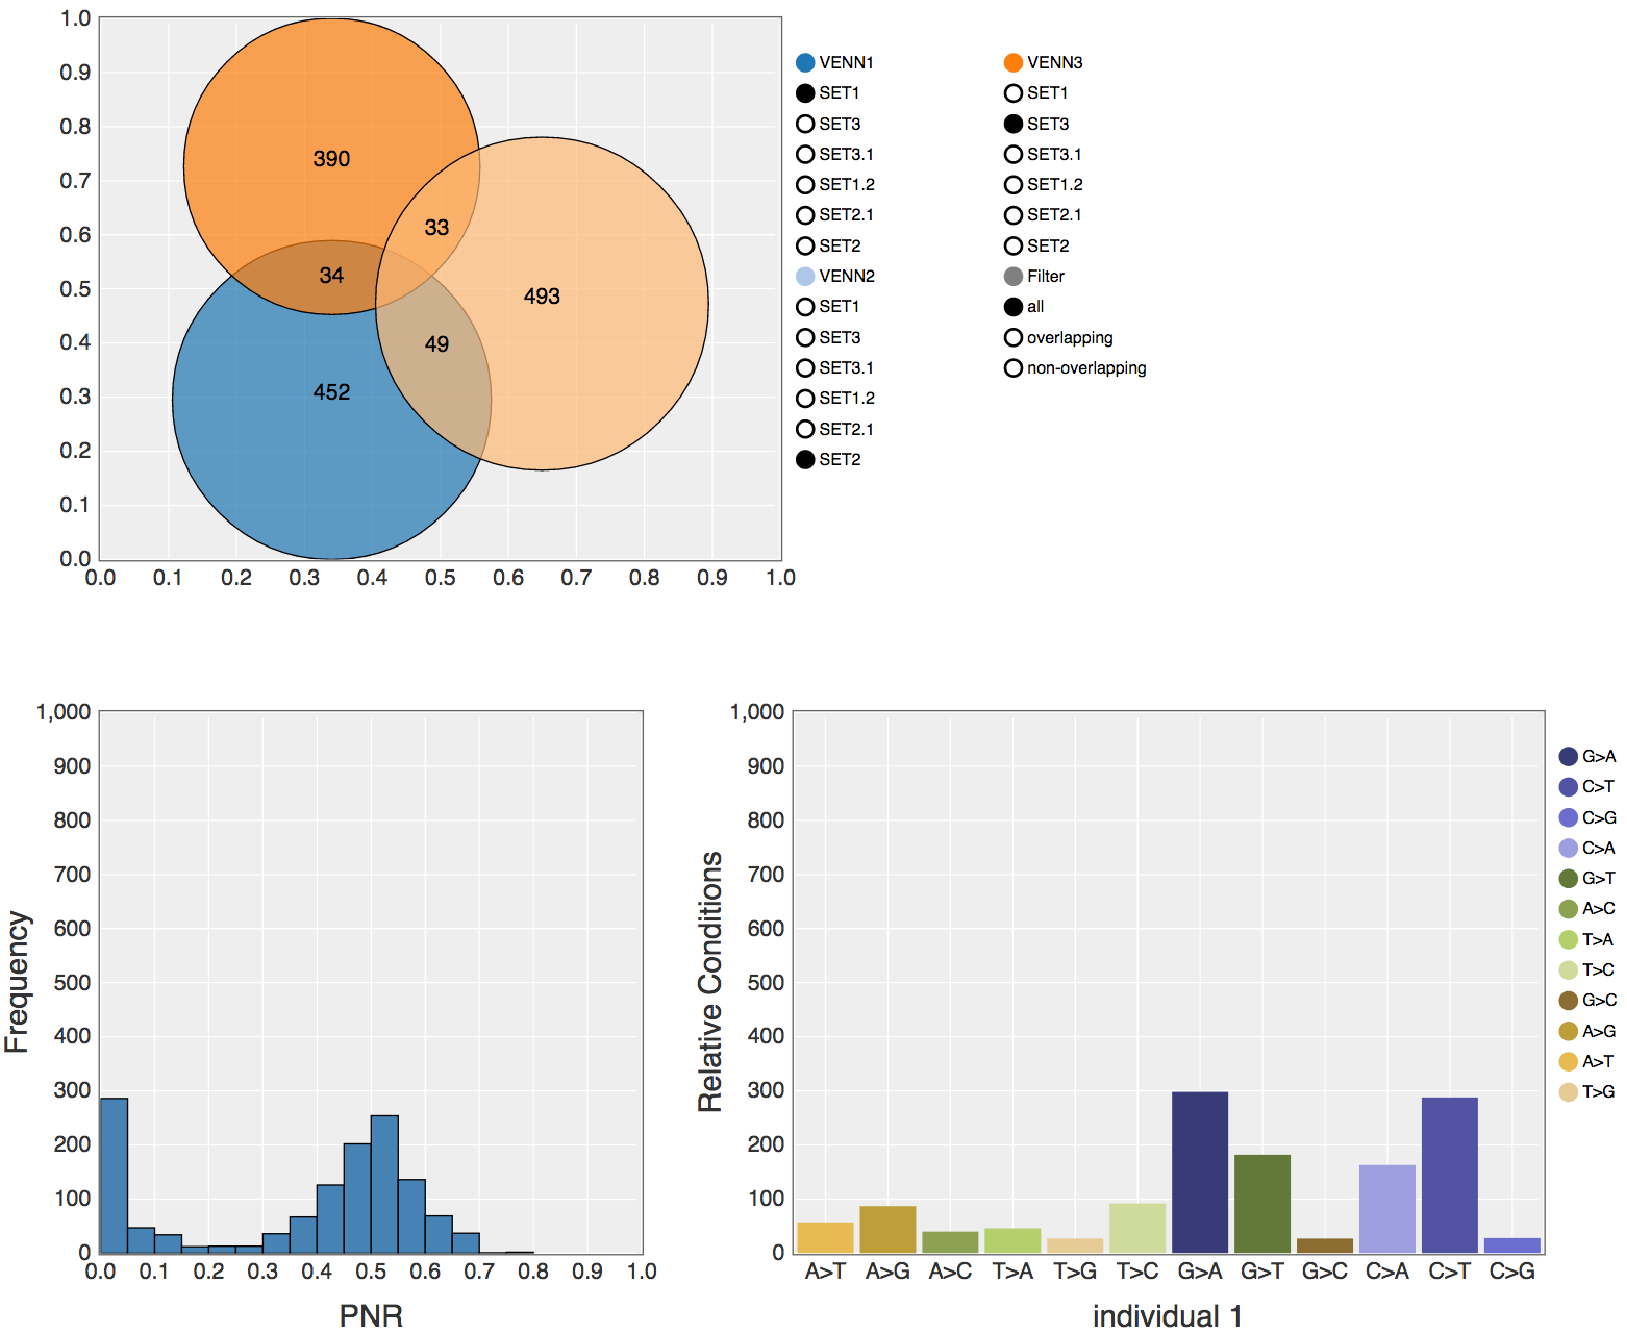
\includegraphics[width=0.75\textwidth]{nyeplot.pdf}
%    \caption{\textbf{Visual analytics in d3.js of mutli-sample variants calls} This example shows the possibilities of d3.js and visual analytics: fast and efficient system-wide exploratory analysis of multiple datasets, including cross-talk between the different modules. An interactive version can be found on \url{www.domitry.com/gsoc/multi_pane2.html}.}
%    \label{fig:nya}
%\end{figure}
%\noindent 
%The heterogeneous samples and datasets of cancer make it one of the most computationally demanding types of integrative biology. \textbf{We propose to use our methods to study to consequences of structural variations at non-coding loci in cancer on other levels.}  These methods will enable research in this technical challenging topic, by decreasing the computational burden of data-handling, and increase the cognitive abilities of the user, by providing integrative visual interfaces. 
%\newpage\subsection*{Originality and innovative character} 
%
%\begin{itemize}
%\item Weinig onderzoek naar NC-SV
%\item awesome locatie en onderzoek
%\item Veel vraag naar integratie
%\item Waar stond RDF vijf jaar geleden? En waar staat RDF nu?
%\item VA is nodig en heul handig, ook voor leken
%\end{itemize}
%
%
%\medskip
%
%\noindent
%
%
%However, there are two main limitations of this relatively young incorporation: a standard language for denoting biological triples (e.g. chromosome locations) is missing and the focus lies at linking database-accessions \citep{Ruttenberg2007}. While the first limitation could also be a strength, as everybody can use their own dialect. However, a standardisation-step will lower the learning-curve, which will enable researchers in all fields of biology to benefit fully from the integrative benefits of the Semantic Web. The second limitation is severely restricting the use of RDF in NGS- and MS-based methods: there are no tools to convert the common formats to triples, like the \textit{Variant Call Format} (VCF) and \textit{Sequence Alignment Format} (SAM). An example of this is  \textit{Bio2RDF}\cite{Belleau2008}: an "\textit{RDFizer}", which converts conventional databases, like the ones from NCBI, to triplestores. One of the leading innovative points of this proposal is the development of methods to handle the NGS- and MS-based formats for use in the Semantic Web. This will result in a broader use of semantic web-technologies for the research community, by enabling the coupling of proprietary NGS- and MS-data to existing RDF-databases.
%\medskip
%
%\noindent
%%added value of linked data visual analytics TOV standaard methodes ( verwijs naar pilot study)
%
%\medskip
%
%\noindent
%
%

%\medskip



%Data acquisition will be performed throughout the study. Ongoing sequencing efforts from the research group of Prof. Dr. Cuppen and collaborators will ensure more than adequate amounts of data will be at our disposal. Due to the accompanied scientific questions of this data, the method-development stages of this study will continue to be focussed and inspired by the end-goal: answering biological questions. Furthermore, continuing the data-acquisition in the second half of the study to will enable us to collaborate with the research community and showcase our innovative technology with new and exciting integrative biology studies.
%\medskip
%
%\noindent
%To ensure the greatest compatibility and effectiveness, tight collaborations will be established between leading RDF-users and -developers in- and outside of biology. Triples for NGS- and MS-based data will be developed, taking into account the most commonly used format first. Since different databases can require a specific triple-structure, RDF-databases will be investigated on their ability to handle the large datasets efficiently, including their in- and output options. Selected research groups in Utrecht will be attracted to provide early feedback-rounds, focussed on usability and compatibility. 
%
%After completion of the triple-development of a data-format (i.e. end-users and the RDF-community have provided positive feedback), development of the conversion-tools is next. In this stage, we seek to expand the capabilities of current leading bioinformatical tools like Sambamba\cite{Tarasov2014} and BIO-VCF\cite{Goto2010}, to capitalise on their multi-core capabilities. Furthermore, we will seek to collaborate with the current (public data-focussed) initiatives, like Bio2RDF\cite{Belleau2008} and BioInterchange\cite{Baran} to ensure software-compatibility and limit redundancy.
%\medskip
%
%\noindent
%The visualisation-subproject will have two phases. In the first phase, we will use a minimalistic model to develop the link between the SPARQL in- and output and \textit{d3.js}-visualisation. The minimalistic model comprises of SNP- and RNA-based visual analytics-based solutions. Resulting methods can be directly used in other projects, focussing on the role of SNPs and transcription(-levels).
%
%After a successful first phase, the second phase will broaden the available visualisations, by creating a modular dashboard. Every module will provide a particular visual (e.g. heat-map, scatter-plot) and will interact with both the SPARQL-input, -output and the other active modules. If a user would, for example, select a specific gene in the scatter-plot, the same data-point will be highlighted in the other modules. The cross-talk between modules has already been implemented in Epiviz2\cite{Chelaru2014}, which is highly appraised for this by its users. The order of development of specific modules will be primarily based on the wants and needs of the community, which will be gathered with the above-mentioned feedback-rounds.
%%\newpage
%\subsection*{Pilot-study}
%
%\newpage
%\section*{Research plan}
%\subsection*{Timetable}
%
%\subsection*{Proposed biological questions}
%Semester four to six will be used to perform multi-level analysis with the resulting methods and tools from the previous three semesters. The overall aim is to combine both proprietary and public data to execute previously impossible analyses. Of the public databases available, the most valuable for our purposes are those, that link omics-data to pathways and ontologies: \textit{Pathway Commons}\cite{Cerami2011} and \textit{Reactome}\cite{Jupp2014} on perturbed pathways in cancer, \textit{RegulomeDB}\cite{Boyle2012} on linking non-coding regions to genes and \textit{Gene Ontology}\cite{Ashburner2000} and \textit{KEGG-pathway}\cite{Kanehisa2000} for general ontologies and pathways. A subset of the addressed questions and proposed analyses is depicted below.
%\renewcommand{\labelenumi}{\roman{enumi}.}
%\begin{enumerate}
%
%








%
%linked data visual analystic zijn in alle velden te grebruiken, die RDf gebruiken. Ook voor bedrijven (pharma!). Super handig!
%
%Vrij snel te incorpporeren: de meeste dingen zijn er al
%
%cancer NC-SV is nog weinig over bekend: mogelijke nieuwe targets voor cancer screening and or treatment: sociaal en pharma.




%-------------------------------------------------------
%	REFERENCE LIST
%----------------------------------------------------------------------------------------

%\begin{thebibliography}{99} % Bibliography - this is intentionally simple in this template

%\renewcommand{\refname}{\LARGE\scshape\centering References} %
%\titleformat*{\section}{\LARGE\scshape\centering}
%\titleformat{\section}[block]{\LARGE\scshape\centering}{\thesection.}{1em}{} % Change the look of the section titles
\begin{tiny}

\bibliography{library}
 \end{tiny}
%\end{thebibliography}
%
%%----------------------------------------------------------------------------------------
%
%%\end{multicols}

\end{document}
